\newcommand{\code}[1]{\texttt{#1}}
\chapter{Il progetto}

\section{Introduzione}
Gli obiettivi pianificati per questo progetto miravano al raggiungimento di un elevato grado qualitativo del software prodotto dall'azienda. Per perseguire tali obiettivi è stato necessario mettere assieme una serie di tecnologie affidabili, in grado di analizzare ciò che viene prodotto, fornendo degli indicatori qualitativi quantificabili e ben dettagliati.

La necessità di perseguire una buona qualità dei prodotti software, nasce dalla richiesta di alcuni clienti di avere dei prodotti conformi rispetto al modello CMMI-DEV.

L'utilizzo delle tecniche che garantiscono la conformità a tale modello, però, è avvenuta in un secondo momento rispetto allo sviluppo iniziale del software per i sistemi \textit{Subsea}. L'azienda non aveva una grande esperienza sul piano della progettazione e dello sviluppo di un software di qualità, ha quindi prodotto una grossa quantità di codice incontrollato e difficile da manutenere. 

Come prima cosa, in continuazione con quanto è stato fatto nello \textit{stage} precedente, mi sono occupato di definire uno standard interno alla Divisione, contenente serie di regole stilistiche per la stesura del codice. Queste regole servono a limitare l'eccessiva libertà con la quale gli sviluppatori producevano il software. Abituati a lavorare in un ambiente disorganizzato, producevano infatti del codice disordinato, poco mantenibile e senza alcuna documentazione. L'applicazione di queste regole, attraverso degli strumenti che segnalano direttamente le non conformità, se da una parte portano ad uno sforzo maggiore richiesto agli sviluppatori, dall'altra garantiscono un codice più ordinato e leggibile. Un codice ben scritto è un prerequisito fondamentale per le successive attività di analisi.

Una volta assicurata una certa qualità sulla scrittura del codice, ho potuto studiare ed analizzare le varie tecnologie da applicare per l'attuazione delle metodologie di analisi statica e dinamica. 
\textit{Pietro Fiorentini S.p.A}, in un'ottica di miglioramento continuo (uno dei pilastri fondamentali sul quale è basata l'azienda), ha visto nelle tecniche di analisi statica e dinamica una possibile area di sviluppo e miglioramento grazie al possibile risparmio di tempo e risorse che si può raggiungere tramite un'applicazione corretta delle tecniche di analisi. Mi sono dunque occupato di studiare quali metodologie fossero le più utili ed interessanti per raggiungere gli obiettivi posti da queste tecniche, ho poi realizzato una struttura di base in grado di elaborare i dati forniti dall'applicazione delle varie metodologie e, infine, ho iniziato l'applicazione di queste tecniche di analisi sul prodotto software.

Una volta definite ed implementate le attività di analisi, avendo quindi generato una base dati iniziale con i risultati delle varie applicazioni di questi metodi, ho potuto rendere quantificabili i risultati ottenuti. Ho perciò scelto ed applicato delle metriche di misurazione di qualità del prodotto software. Grazie a queste metriche è possibile capire immediatamente quanto il prodotto stia migliorando rispetto alle versioni precedenti nelle quali non era stato previsto alcun tipo di controllo. Con queste misurazioni è possibile anche dimostrare al cliente finale che il software prodotto è sempre controllato, fornendo un risultato tangibile di qualità.

%\section{Pianificazione}
%\textcolor{OliveGreen}{\textbf{Definisco il metodo con cui mi sono approcciato per analizzare, documentare e sviluppare le quattro fasi principali del progetto.}}

Il progetto di stage è articolato dunque in quattro fasi principali: analisi dello stile di codifica, analisi statica del codice, analisi dinamica e misurazione delle metriche di qualità. 

Per ognuna di queste fasi, in linea con il modello di ciclo di vita del software adottato dall'azienda, sono state pianificate delle attività principali da eseguire. Dopo una prima analisi preliminare delle richieste del progetto, dell'architettura esistente, e di quanto era già stato prodotto dagli \textit{stage} precedenti, sono passato ad analizzare e a pianificare in dettaglio l'utilizzo dei vari strumenti, per poter garantire una soluzione ottimale alle varie richieste. A seguito di questa pianificazione, basata anche sull'utilizzo di \textit{best-practice} esistenti, ho continuato con la realizzazione e l'integrazione degli strumenti con i sistemi di gestione di processi già utilizzati dall'azienda.

In questo capitolo verranno esplicitate nel dettaglio tutte le fasi del progetto e gli aspetti fin qui accennati. Per ogni fase saranno specificate le motivazioni delle scelte effettuate, i principi base che hanno supportato l'applicazione degli strumenti, le regole, i controlli effettivamente implementati e come questi strumenti sono stati eseguiti ed integrati nel sistema esistente.



%Per garantire un adeguato livello qualitativo del software all'interno dei sistemi Subsea, alcuni clienti hanno richiesto la conformità rispetto al modello CMMI-DEV. 
%
%Il mio progetto si accoda ad una serie di altri \textit{stage} che hanno avuto come obiettivo principale l'implementazione dei sistemi per la gestione dei processi che fossero conformi a tale modello.




\section{Stile di codifica}
%\textcolor{OliveGreen}{\textbf{Scelte e motivazioni per l'utilizzo di tools di analisi dello stile di codice, associate ad alcune best-practice esistenti. }}

Uno stile di codifica unificato tra tutti i programmatori è un prerequisito fondamentale per molte ragioni: la prima  riguarda il fatto che, in tutto il ciclo di vita di un prodotto \textit{software}, la maggior parte del tempo viene dedicata alla manutenzione. Solitamente questa attività viene affidata a una persona diversa dallo sviluppatore che ha scritto quel particolare pezzo di codice, e avere uno stile di scrittura uniforme e aderente anche ad alcuni standard, facilita molto questa fase.

Condividere uno standard comune di codifica comporta anche molti altri benefici: aumenta la condivisione e la comunicazione tra i diversi sviluppatori, dà la possibilità agli altri membri del reparto Ricerca e Sviluppo con competenze informatiche di visionare ed eventualmente modificare il codice prodotto, evita molti errori banali aumentando così sia la qualità generale del codice che il lavoro di squadra.

Avere un numero fissato di regole e convenzioni, poi, aiuta molto le attività di verifica e validazione infatti, avere un codice scritto sempre nello stesso modo e che quindi sia standardizzato permette di facilitare e velocizzare la stesura e l'automazione delle procedure di test.

L'utilizzo di uno standard di scrittura è stato richiesto, da parte dell'azienda, anche per garantire un'adeguata documentazione del software prodotto. Questa richiesta nasce perché, all'inizio della realizzazione del progetto \textit{software}, era stata lasciata la massima libertà di lavoro agli sviluppatori, che hanno prodotto una grande quantità di codice senza nessuna documentazione. Così facendo, alla prima occasione in cui è stata richiesta una manutenzione, il reparto di Ricerca e Sviluppo si è trovato davanti a notevoli difficoltà, e si è accorto che la qualità del \textit{software} prodotto era particolarmente bassa; ha quindi deciso di porre delle regole ben precise per non ripetere gli errori passati.

Per garantire un alto livello qualitativo dei processi e per specificare in dettaglio le scelte di progettazione effettuate, ho prodotto un documento denominato \textit{Code style guide}. Questo documento è pensato per raccogliere tutte le regole di stile previste ed implementate specificandone le motivazioni e i dettagli implementativi. Una prima bozza di documento era già stata scritta nello \textit{stage} precedente. Mi sono occupato principalmente di estendere e modificare alcune delle regole di stile pianificate.

\subsection{Principi base}
Per garantire un buon prodotto software è necessario pianificare correttamente cosa si andrà a sviluppare. Per facilitare questa fase è opportuno che gli sviluppatori prendano in considerazione questi principi prima di cominciare a produrre il codice. 

L'utilizzo di questi principi, accompagnato da uno stile di codifica ben definito, garantisce una buona qualità del software prodotto e facilità le successive fasi di analisi.

\begin{itemize}
\item[] \textbf{KISS} \textit{Keep It Simple Stupid} vuole suggerire al programmatore di sviluppare i vari metodi mantenendo un livello di complessità minimo. Ogni attività da produrre deve essere la più semplice possibile massimizzando la coesione tra le componenti e abbassando l'accoppiamento.

\item[] \textbf{SOLID} \textit{SOLID} è un acronimo che fornisce cinque principi fondamentali per una buona progettazione. Questi garantiscono un codice flessibile, robusto, mantenibile e riutilizzabile.
\begin{itemize}
\item[•] \textbf{\textit{Single Responsability Principle}}: ogni classe dovrebbe avere una ed una sola responsabilità;

\item[•] \textbf{\textit{Open-Close Principle}}: un'entità \textit{software} dovrebbe essere aperta alle estensioni ma chiusa alle modifiche;

\item[•] \textbf{\textit{Liskov's Substitution Principle}}: gli oggetti dovrebbero poter essere sostituiti con dei loro sottotipi, senza alterare il comportamento del programma che li utilizza;

\item[•] \textbf{\textit{Interface Segregation Principle}}: sono preferibili più interfacce specifiche, che una singola generica;

\item[•] \textbf{\textit{Dependency Inversion Principle}}: una classe dovrebbe dipendere dalle astrazioni, non da classi concrete.
\end{itemize}

\item[] \textbf{DRY} \textit{Don't Repeat Yourself} vuole suggerire al programmatore di evitare di scrivere più volte le stesse linee di codice. È meglio infatti massimizzare il riutilizzo rispetto ad utilizzare una ripetizione del codice.
\end{itemize}

\subsection{Automazione di controlli}
Il linguaggio principale con cui viene sviluppato il \textit{software} per i misuratori di flusso è il \textit{C++}. Sono state dunque definite diverse categorie di controlli sull'analisi dello stile di codifica.

\begin{itemize}
\item[•] \textbf{Definizione dei nomi}: è importante assegnare un nome corretto e significativo a metodi, classi e attributi, in modo tale da facilitare la comprensione del loro funzionamento e del loro scopo. Riporto di seguito le più significative tra le regole implementate:
\begin{itemize}
\item[•] \textbf{Nome delle funzioni}: il nome , come detto, deve essere significativo rispetto allo scopo della funzione e non deve contenere lettere maiuscole. I nomi delle componenti, poi, devono essere separati da un \textit{"underscore"};

\item[•] \textbf{\#define e macro}: l'utilizzo delle \textit{keyword} \#define e macro deve essere limitato solamente all'interno dei file di intestazione (\textit{.h});

\item[•] \textbf{Nomi dei file}: i nomi dei file non devono contenere spazi;

\item[•] \textbf{Nomi variabili puntatore}: il simbolo * del puntatore deve essere posto vicino al tipo della variabile. Il nome del puntatore deve cominciare con: "p\_";

\item[•] \textbf{Nomi degli array}: il nome degli array deve cominciare con: "a\_".
\end{itemize}

\item[•] \textbf{Definizione della formattazione}: definire una indentazione e un \textit{pattern} di formattazione comuni, in modo tale da avere uno stile unico per tutto il codice sorgente scritto. A titolo esemplificativo, riporto alcune delle regole implementate:
\begin{itemize}
\item[•] \textbf{Lunghezza massima riga}: ogni riga di codice non deve superare i 120 caratteri, per garantire una buona lettura;

\item[•] \textbf{Lunghezza massima file}: ogni file non deve contenere più di 1000 righe di codice

\item[•] \textbf{Evitare le negazioni nella forma ridotta}: utilizzare le negazioni della forma ridotta diminuisce la leggibilità del codice.
\end{itemize}

\item[•] \textbf{Definizione della documentazione}: per garantire una corretta manutenibilità, e per permettere ad altre persone di leggere e capire il codice scritto, è necessario commentare adeguatamente il codice scritto. A questo scopo è importante porre la giusta attenzione a:

\begin{itemize}
\item[•] \textbf{Intestazione file}: ogni file deve contenere un commento di intestazione che ne specifichi lo scopo, l'autore, e il nome. Sarà compito del sistema di versionamento SVN aggiornare automaticamente i campi dati relativi alle modifiche effettuate dopo ogni commit;

\item[•] \textbf{Intestazione funzioni}: per ogni funzione sviluppata devono essere descritti lo scopo, i parametri che richiede in input e la tipologia di risultato che ritorna. 
\end{itemize}
\end{itemize}

\subsection{Strumenti utilizzati}
%\textcolor{OliveGreen}{\textbf{Descrivo quali sono gli strumenti e come sono stati implementati}}
Per effettuare un'analisi completa e approfondita dello stile di codifica, mi sono servito di alcuni strumenti \glossaryItem{open source} già presenti sul mercato. Si tratta principalmente di strumenti che eseguono un analisi testuale del codice confrontando quanto è stato scritto con errori tipici noti.

L'attività che ho svolto è stata articolata in due momenti: inizialmente ho ricercato gli strumenti più adatti per segnalare le regole pianificate (vedi 3.2.2), successivamente, dopo averli testati, ho analizzato i dati restituiti. Questi strumenti generano infatti un'enorme quantità di risultati e segnalano migliaia di errori; molto spesso, però, sono solo falsi positivi. Questa bassa accuratezza è alla base della sfiducia verso tali strumenti e ho voluto quindi lavorare sui loro output con lo scopo di garantire una certa affidabilità alle segnalazioni che verranno effettuate agli sviluppatori, quando li utilizzeranno in modo sistematico. Tra i principali strumenti studiati vi sono:
\begin{itemize}
\item[•] \textbf{Uncrustify}: strumento gratuito che permette di definire delle regole di stile, indentare e strutturare i file a proprio piacere. Si occupa principalmente di analizzare e correggere la formattazione del codice sorgente sviluppato.

\item[•] \textbf{Vera++}: è uno strumento per la verifica e l'analisi del codice sorgente scritto in \textit{C++}. Si tratta di un \textit{parser} che analizza le principali \textit{keyword} tipiche del \textit{C++}, verificando se il loro utilizzo e la loro posizione rispettano le regole definite dal linguaggio. Si occupa principalmente di analizzare l'utilizzo e la definizione dei nomi delle varie componenti \textit{software} realizzate.
\end{itemize}

Grazie all'integrazione di questi due strumenti, e ad altri \textit{parser} testuali più semplici, ho potuto ricoprire al meglio le regole pianificate di analisi dello stile di codifica.

Il lavoro che ho fatto di aggregazione fornisce una base solida che può essere facilmente ampliata aggiungendo ulteriori strumenti esterni di analisi.

Oltre alla realizzazione di strumenti per l'analisi, ho creato uno \textit{script} eseguibile sia in ambiente \textit{Linux} che in ambiente \textit{Windows} in grado di correggere in modo automatizzato alcuni degli errori segnalati. La responsabilità dell'applicazione di questo strumento viene lasciata allo sviluppatore il quale può confermare se le modifiche apportate siano veramente volute e necessarie.

\section{Analisi statica}
%\textcolor{OliveGreen}{\textbf{Scelte e motivazioni per l'utilizzo di tools di analisi statica, associate ad alcune best-practice esistenti.}}

Nessun linguaggio di programmazione può garantire la verificabilità di ciò che è stato scritto. Visto l'aumento dei software che incorporano funzionalità strategiche o critiche per la sicurezza, ogni falla nel sistema può causare ingenti danni economici e di immagine. È nata così la necessità di avere un codice ben strutturato per rendere efficaci le attività di verifica, in modo da eliminare qualsiasi situazione critica che possa creare problemi. Lo scopo dell'analisi statica è proprio quello di trovare e notificare eventuali errori sulla struttura di un programma. Solitamente questo tipo di analisi viene utilizzata per verificare la corretta applicazione degli standard di codifica, per analizzare la complessità con la quale viene scritto il \textit{software} oppure per identificare anomalie o difetti.

L'analisi statica aiuta i verificatori a trovare eventuali errori prima che il compilatore li trasformi in bug eseguiti a \textit{run-time}. Alcuni esempi di questi errori, dati molto spesso da inesperienza o distrazione, sono l'utilizzo di una variabile non inizializzata, oppure l'indicizzazione di un array oltre al limite in cui è stato allocato. Con l'esperienza degli sviluppatori l'incidenza di questi \textit{bug} diminuisce, ma resta comunque estremamente frustrante e costosa da sistemare.

Questa tecnica si basa sull'analisi del codice in modo statico, senza la sua esecuzione, attraverso un attento esame dell'intero codice sorgente. Grazie a questa analisi è possibile diagnosticare: violazioni di regole o convenzioni necessarie per la corretta esecuzione del programma, assicurare una buona manutenibilità, evitare uno stile di programmazione poco sicuro.

\begin{figure}[H]
  \centering
  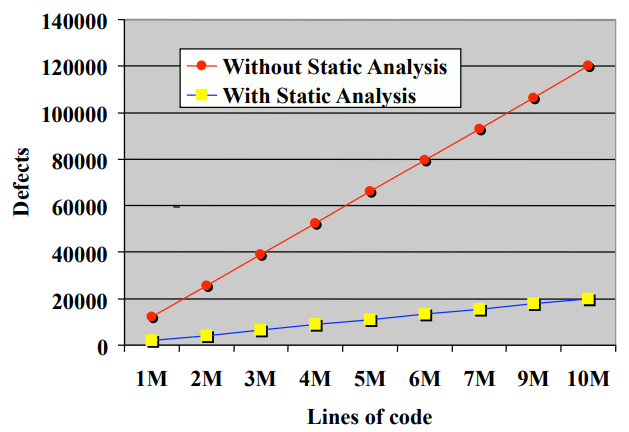
\includegraphics[scale=0.6]{static.PNG}
  \caption{Efficacia analisi statica - Tratta da: Capers Jones, Software Productivity Group}
\end{figure}

\textit{"60\% of the software faults that were found in released software products could have been detected by means of static analysis"} - Bloor Research Ltd., UK CAST Tools report of 1996

Utilizzare l'analisi statica è un'attività utile sia per il responsabile di progetto che per gli sviluppatori. Questo tipo di analisi, infatti, aiuta il responsabile a ridurre i rischi e i costi derivati da eventuali errori commessi durante lo sviluppo, e riduce i costi e i tempi per la verifica del codice. Lo sviluppatore, invece, è avvantaggiato durante la fase di \textit{debugging} in quanto si previene la formazione di \textit{bug} rendendoli visibili prima che diventino difficili da trovare.

La richiesta da parte dell'azienda di implementare gli strumenti di analisi statica, nasce dalla possibilità di ridurre i costi e il tempo speso per correggere gli errori. Per rendere davvero efficace questa tecnologia, però, deve essere una parte integrante del ciclo di vita del software, solo in questo modo si riesce a massimizzare i risultati.

Lo scopo di questa fase di progetto sono state dunque la ricerca e l'implementazione degli strumenti utili per l'analisi statica, integrandoli a pieno con i sistemi di integrazione continua esistenti.

Per garantire un alto livello qualitativo dei processi e per specificare in dettaglio le scelte di progettazione effettuate, ho prodotto un documento denominato \textit{Code static analysis}.
Lo scopo di questo documento è descrivere le metodologie utilizzate di analisi statica del software, definendo le \textit{best-practice} seguite in modo tale da limitare i problemi durante le fasi di sviluppo e debugging. Mi sono occupato dell'intera stesura del documento fornendo anche i dettagli degli strumenti sviluppati

\subsection{Principi base}
Per semplificare e rendere più efficienti gli automatismi degli strumenti di analisi statica, abbiamo deciso di sviluppare questi strumenti basandoci sulle seguenti regole, e suggerendo anche agli sviluppatori di applicarle. 

\begin{itemize}


\item[] \textbf{The power of Ten}: è un documento stilato nel 2006 da \textit{Gerard J. Holzmann} che elenca 10 regole per scrivere codice in C. Alcune di queste regole sono simili a quanto già definito durante la fase di analisi dello stile di codifica poichè si basano sugli stessi principi.

\begin{enumerate}
\item \textbf{Utilizzare un controllo di flusso semplice}: non utilizzare costrutti \code{goto, setjmp, longjmp} ed evitare la ricorsione, sia diretta che indiretta. Questa regola rende il codice più chiaro e più semplice, aiutando i verificatori e le persone esterne che potranno in futuro dover modificare il codice scritto.

\item \textbf{Porre un limite superiore ai cicli}: questa regola assicura che non ci sia codice che abbia un comportamento inaspettato o che corrompa aree di memoria esterne al suo \textit{scope}. I limiti dovranno essere testati staticamente.

\item \textbf{Non usare allocazione dinamica della memoria dopo l'inizializzazione}: questa regola è fondamentalle per ambienti in cui è richiesto un alto grado di sicurezza e affidabilità. 

\item \textbf{Limitare le funzioni a 60 righe di codice}: questa regola aiuta la comprensibilità del codice. Ogni funzione deve essere contenuta in una singola pagina per garantire una buona visibilità.

\item \textbf{Nel codice devono essere presenti almeno due asserzioni per funzione}: queste asserzioni devono proteggere da situazioni anomale e non provocare \textit{side-effect}. Tramite le asserzioni, tipicamente test booleani, si intende testare pre-  e post- condizioni delle funzioni, dei parametri, dei valori di ritorno e gli invarianti dei vari cicli.

\item \textbf{Tutti gli oggetti e le variabili devono essere dichiarati con il minor scope possibile}: questa regola restringe al minimo l'area in cui un oggetto può essere modificato e corrotto, aumentando la sicurezza del sistema e semplificando il lavoro di verificatori e \textit{debugger}.

\item \textbf{Ogni funzione chiamante deve controllare i valori restituitele dalle funzioni chiamate e ogni funzione chiamata deve controllare la validità dei parametri passatele dal chiamante}: questa regola di programmazione aiuta ad aumentare la sicurezza del sistema perché verifica i valori passati all'interno del codice del programma.

\item \textbf{L'uso del pre-processore deve essere limitato all'inclusione di file \textit{header} e alla definizione di semplici macro}: questa regola è posta per evitare che il numero di casi da testare aumenti esponenzialmente all'aumentare della clausole condizionali.

\item \textbf{L'uso dei puntatori deve essere limitato e non è permesso più di un livello di deferenziazione}: questa regola è stata posta perché i puntatori sono spesso usati in modo scorretto e provocano molti errori di programmazione.

\item \textbf{Tutto il codice prodotto deve essere compilato, fin dal primo giorno, con tutti i warning attivi. Il codice deve compilare senza warning}: questa regola incentiva la scrittura di codice corretto e suggerisce di utilizzare l'integrazione continua
\end{enumerate} 

\item[] \textbf{MISRA C - 2004}: è un insieme di linee guida di sviluppo software per linguaggio di programmazione \textit{C} sviluppato da MISRA \textit{(Motor Industry Software Association)}. Il suo scopo è di facilitare la sicurezza, la portabilità e l'affidabilità del codice nel contesto dei \glossaryItem{sistemi embedded}.
MISRA C non è uno standard \glossaryItem{open source}, però ho deciso di utilizzarlo in quanto viene fornito uno strumento di analisi che fa riferimento a queste regole, da parte del compilatore IAR.
\end{itemize}

\subsection{Tecniche di analisi}
A seconda della tipologia di controllo che si vuole implementare e della sua esecuzione, vi sono diverse tipologie di approcci da utilizzare.

Una tipologia di analisi si fa tramite metodo di lettura, cioè analizzando il codice con tecniche di \textit{Inspection o Walkthorugh}. Queste tecniche prevedono una lettura mirata o a largo spettro di tutto il codice prodotto da parte di un team di persone formato da verificatori e sviluppatori. 

Questi metodi, se condotti nel modo corretto, producono dei buoni risultati con una buona affidabilità, però sono stati scartati in quanto la loro realizzazione richiederebbe del personale altamente specializzato che al momento manca all'interno dell'organico della divisione, e un tempo troppo elevato per analizzare e correggere completamente tutto il codice.

Per questo motivo abbiamo deciso di utilizzare dei metodi formali. Questi prevedono l'utilizzo di tecniche che possono essere automatizzate, rendendo più semplice il lavoro dei verificatori. Alcune delle tecniche analizzate sono:
\begin{itemize}
\item[•] \textbf{Analisi del flusso di controllo}, questa tipologia di analisi assicura che il codice sorgente venga eseguito nella giusta sequenza e che tutto il codice scritto venga eseguito correttamente. Non esisteranno quindi più pezzi di codice irraggiungibili oppure cicli infiniti che non terminano mai.

Alcune delle regole che possono essere implementate riguardano: la verifica che non ci sia codice irraggiungibile, assicurare la terminazione dei cicli, garantire il corretto utilizzo dei puntatori, evitando i puntatori a \textit{null}.

\item[•] \textbf{Analisi del flusso dei dati}, questa tipologia di analisi identifica se alcune parti del programma non sono conformi alle regole del linguaggio di programmazione. Controlla ad esempio se vengono sovra-scritte delle variabili senza verificarne prima il valore.

Alcune delle regole che possono essere implementate riguardano: il controllo dei tipi in un'associazione tra variabili, l'utilizzo di variabili non inizializzate.

\item[•] \textbf{Analisi i limite}, questa tipologia di analisi viene utilizzata per assicurare che i dati elaborati dal programma rimangano entro i limiti dichiarati dalla precisione del proprio tipo.

Alcune delle regole che possono essere implementate riguardano: il controllo dell'indicizzazione negli array, assegnazioni sospette o \textit{cast} pericolosi.

\item[•] \textbf{Analisi del flusso delle informazioni}, questa tipologia di analisi determina quali dipendenze vi sono tra i parametri in ingesso di una funzione e i risultati attesi. Sono permesse solamente le dipendenze descritte nelle specifiche.

\end{itemize}

\subsection{Automazione di controlli}
Per facilitare l'inizio delle attività di analisi statica, ho deciso, in accordo con il tutor aziendale, di implementare solamente alcune delle regole inizialmente analizzate, per far capire l'importanza di questo tipo di analisi agli sviluppatori senza però scoraggiarli, limitando così gli errori riportati nei report.
Alcune di queste regole sono:
\begin{itemize}
\item[•] \textbf{Possibile dereferenziazione di un puntatore a \code{NULL}}: dereferenziare un puntatore a \code{NULL} solitamente comporta la lettura o scrittura di un'area di memoria non mappata, provocando un \textit{segmentation fault} o una violazione di accesso;

\item[•] \textbf{Array oltre al limite}: assicura che gli indici utilizzati per l'accesso ai dati siano entro ai limiti della dimensione dell'array;

\item[•] \textbf{MISRA C rule 9.1}: assicura che a tutte le variabili sia assegnato un valore prima del loro utilizzo;

\item[•] \textbf{MISRA C rule 14.1}: assicura che non ci sia del codice irraggiungibile;

\item[•] \textbf{MISRA C rule 14.6}: assicura che per ogni iterazione vi sia al massimo un solo \code{break} per terminare il ciclo. Questa regola garantisce una buona struttura del programma;


\end{itemize}

\subsection{Strumenti utilizzati}
%\textcolor{OliveGreen}{\textbf{Descrivo quali sono gli strumenti e come sono stati implementati}}
La tipologia di strumenti utilizzati per l'esecuzione dei test di analisi statica è denominata \code{lint}. Si tratta di uno strumento simile ad un compilatore che scansiona i file sorgenti \textit{C e C++}, controllando se sono sintatticamente corretti.

I principali strumenti che ho utilizzato ed integrato per avere un unico sistema di esecuzione per l'analisi statica del software sono:

\begin{itemize}
\item[•] \textbf{CppCheck}: è uno strumento di analisi statica per codice C/C++ che fornisce un'analisi del codice in grado di rilevare dei bug. L'analisi effettuata da questo strumento si concentra soprattutto sulla rilevazione di componenti non ben definite e sull'utilizzo di costrutti pericolosi utilizzati in fase di codifica.

\item[•] \textbf{IAR MISRA C}: il compilatore IAR contiene una licenza per visionare e segnalare eventuali non conformità rispetto ad un set di regole di MISRA C. Queste regole si sono diffuse in tutto il mondo e in vari segmenti del settore \textit{embedded}
\end{itemize}.

\section{Analisi dinamica}
%\textcolor{OliveGreen}{\textbf{Scelte e motivazioni per l'utilizzo di tools di analisi dinamica, associate ad alcune best-practice esistenti.}}

L'analisi dinamica ha lo scopo di verificare il comportamento del codice durante la sua esecuzione. Il processo di attuazione di questo tipo di analisi può essere suddiviso in diversi passaggi: preparare i dati da utilizzare come input, eseguire i programmi di test, analizzare i risultati prodotti.

Questa tipologia di analisi copre un vasto campo applicativo che non può essere coperto del tutto in un singolo progetto di \textit{stage} come quello da me intrapreso. Mi sono dunque focalizzato sull'analisi delle possibili applicazioni provando i vari strumenti esistenti sul mercato e selezionando quelli che, a mio avviso, sono più validi. Una volta selezionati, ho creato un'infrastruttura in grado di analizzare del codice sorgente, eseguire dei test pianificati e produrre in modo automatizzato i risultati. Ho applicato questa infrastruttura ad una piccola versione di prova del software prodotto dall'azienda, per dimostrare che ciò che viene solitamente studiato è realmente applicabile e produce sin da subito dei buoni risultati.

Per garantire un alto livello qualitativo dei processi e per specificare in dettaglio le scelte di progettazione effettuate, ho prodotto un documento denominato \textit{Code dynamic analysis}.
Lo scopo di questo documento è definire le tecnologie applicate per l'analisi dinamica del software, in modo tale da evitare errori a \textit{run-time} e \textit{bug}. Mi sono occupato dell'intera stesura del documento descrivendo le scelte progettuali e dettagliando gli strumenti realizzati per favorire una futura crescita di questo tipo di analisi.

\subsection{Principi base}

Per comprendere al meglio l'ambito e i limiti dei test e per eseguirli nella maniera corretta, durante la fase di progettazione e selezione delle tecnologie da adottare per esaminare il software, mi sono basato sul documento \textit{Seven principles of doftware testing} realizzato da Bernard Meyer.

\begin{enumerate}
\item \textbf{Definizione}: "Testare un programma significa cercare di farlo fallire". Questo principio mantiene il processo di testing focalizzato: il suo unico obiettivo è scoprire gli errori che innescando dei fallimenti. La definizione ci ricorda anche che il testing, a differenza del debugging, non si occupa di correggere i guasti, ma solo di trovarli.

\item \textbf{Test vs specifiche}: "I test non possono sostituire le specifiche." Il pericolo di credere che un insieme di test possa servire come specifica è evidenziato da diversi disastri software che sono accaduti, questo perché nessuno aveva pensato a casi estremi. 

Anche se le specifiche non garantiscono una copertura massima di tutti i casi possibili, almeno implicano uno sforzo di generalizzazione. In particolare, le specifiche possono servire a generare test, il contrario però, non è possibile.

\item \textbf{Test di regressione}:  "Qualsiasi test che viene fallito, deve essere mantenuto all'interno della \textit{test-suite}" Questo principio copre tutti i guasti che si verificano durante lo sviluppo e il test. Suggerisce degli strumenti per trasformare un'esecuzione fallita in un test riproducibile.

\item \textbf{Applicazione degli oracoli}  "Gli oracoli dovrebbero essere una parte integrante del codice sviluppato. Determinare il successo o il fallimento del test dovrebbe essere un processo automatico che consiste nel monitorare la soddisfazione delle post-condizioni durante l'esecuzione." L'esecuzione di un test è utile solo se è possibile determinare, in maniera automatica (attraverso oracoli) e senza ambiguità, il risultato finale.

\item \textbf{Esecuzione automatica e manuale dei test}:  "Un processo di test efficace deve includere sia test prodotti manualmente che automaticamente." 

I test manuali hanno una buona profondità: riflettono i ragionamenti degli sviluppatori sul dominio del problema e della struttura dei dati. 

I test automatici hanno una buona capienza: provano molti valori, inclusi gli estremi che gli umani potrebbero perdere.

\item \textbf{Valutazione empirica delle strategie di test}: "Valutare le diverse strategie di test attraverso criteri obiettivi ed espliciti per garantire la riproducibilità dei risultati." I test sono difficili da ricercare e attuare; non tutte le idee intelligenti si dimostrano utili quando sottoposte a una valutazione obiettiva. Un tipico esempio è il test casuale. Le misure oggettive, come il numero di errori rilevati, mostrano che i test casuali spesso producono risultati migliori rispetto ad altre idee apparentemente più intelligenti.

\item \textbf{Criteri di valutazione}: "La proprietà più importante di una strategia di test è il numero di errori scoperti in funzione del tempo." Vogliamo trovare tutti i difetti, non solo uno, l'idea è che il primo errore verrà corretto e il criterio applicato ancora. Ma i difetti successivi potrebbero essere di natura diversa; un processo automatizzato deve innescare quanti più errori possibili, non fermarsi al primo. 

\end{enumerate}

\subsection{Tecniche di test}
Uno dei principali obiettivi del \textit{ testing} è la ricerca del maggior numero possibile di errori all'interno di un programma. Queste tecniche provano a "rompere" il programma da testare, attraverso un approccio il più sistematico possibile, in grado quindi, di garantirne la riproducibilità. 

La classificazione delle tecniche di analisi ricercate, da applicare al software realizzato dall'azienda,  si basa sulle specifiche, sulla struttura del codice e sull'ambito di utilizzo dell'intero prodotto. Alcune delle tecniche di test adottate sono:

\begin{itemize}
\item[•] \textbf{Test dei valori limite}: vengono scelti dei valori vicini ai limiti di dominio delle variabili utilizzate in \textit{input}. In questo modo e possibile verificare la robustezza del codice, verificando se il programma è in grado di elaborare degli \textit{input} inaspettati o errati.

Ho deciso di implementare questa tecnica di analisi dinamica in quanto, trattandosi di un software che contiene dei contatori che misurano la quantità di petrolio estratta, ed elaborando i dati su sistemi \glossaryItem{embedded}, si corre il rischio di raggiungere i limiti massimi previsti dal tipo di dato scelto durante la fase di programmazione. Questo problema comporterebbe il rischio di raggiungere i valori di \textit{overflow o underflow} dei contatori, generando così grossi problemi sui risultati della misurazione.

\item[•] \textbf{Test random}: vengono generati dei test \textit{random}, passando come valori di \textit{input} delle funzioni dei dati \textit{random}, in modo tale da verificare se il comportamento di tale funzione è sempre quello voluto.

Ho deciso di implementare questa tipologia di analisi dinamica per simulare il malfunzionamento di uno dei sensori \textbf{hardware} esistenti. In caso di guasto di uno di questi sensori, potrebbero essere passati dei valori \textit{random} alle funzioni, e voglio garantirne sempre il corretto funzionamento.

\item[•] \textbf{Test dei mutanti}: vengono generati dei test per verificare se le funzioni sono state progettate correttamente. Effettuare test sui mutanti vuol dire, durante l'analisi di una funzione, mutare il codice e confrontare poi il comportamento della funzione originale e di quella mutata, se è diverso la funzione è stata progettata bene, altrimenti no.

Si tratta di una tipologia di test che serve a verificare la robustezza del codice.
\end{itemize}

Per fornire all'azienda una metodologia solida per la pianificazione, la realizzazione e l'implementazione dei test, ho deciso di adottare il modello a V.

\begin{figure}[H]
  \centering
  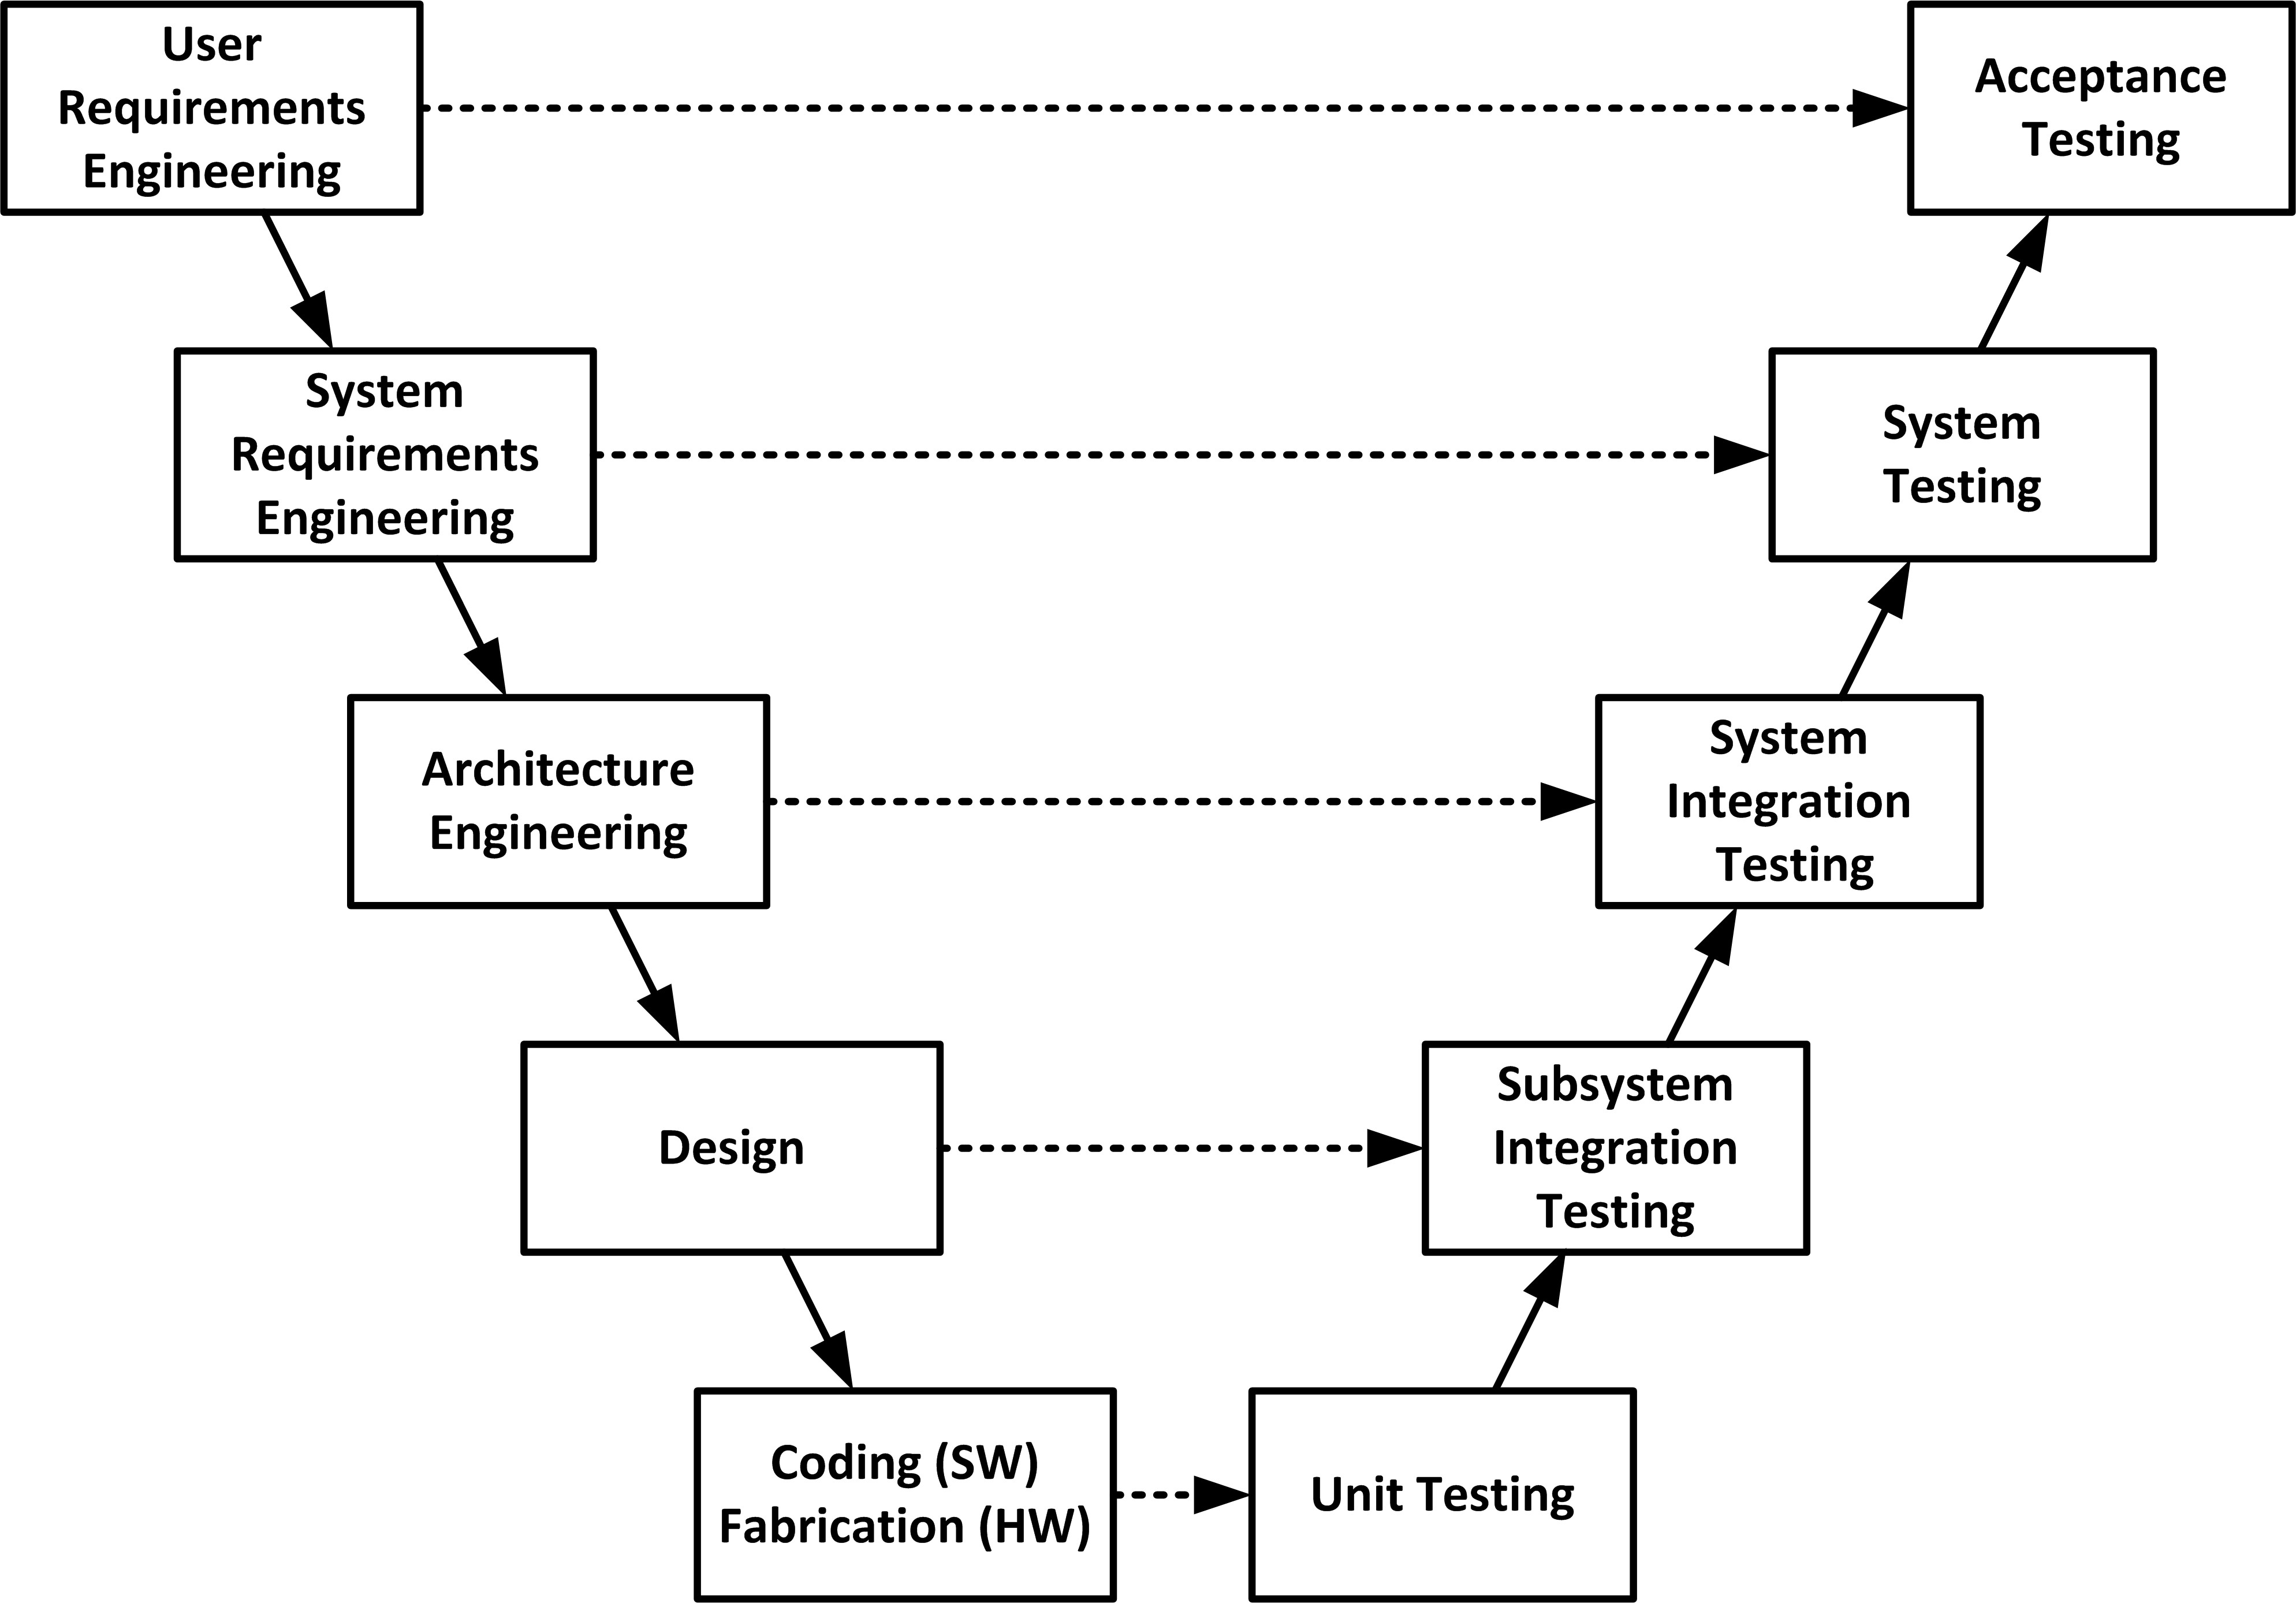
\includegraphics[scale=0.6]{vmodel.jpg}
  \caption{Modello a V}
\end{figure}

In questo modello vengono descritti i passi e le sequenze che devono essere seguite durante l'esecuzione dei test. Le diverse tipologie di test sono state raggruppate in diversi livelli tra cui:
\begin{itemize}
\item[•] \textbf{Test di unità}: verificano il funzionamento di ogni singolo elemento \textit{software} separato degli altri;

\item[•] \textbf{Test di integrazione}: verificano la corretta iterazione tra le diverse componenti \textit{software};

\item[•] \textbf{Test di sistema}: verifica il funzionamento corretto di intere aree del sistema.
\end{itemize}

\subsection{Attività di test}

Una volta definiti i concetti principali che stanno alla base dei test, e le varie tecniche adottate, è necessario integrare quanto è stato sopra descritto in un processo definito e controllato. È opportuno dunque definire un processo che supporti le attività di test e fornisca ai verificatori ed agli sviluppatori informazioni riguardanti la pianificazione dei test, la verifica e la valutazione degli output. In questo modo, grazie ad un processo controllato, è possibile garantire che gli obiettivi dei test sono raggiunti in un modo economicamente conveniente.

Per assicurare un'esecuzione disciplinata e sistematica dei test è stato definito un \textit{Test Plan}. Si tratta di un documento ufficiale che definisce le strategie di test che possono essere attuate, l'ambiente di esecuzione dei vari test, e tutti i passi che devono essere attuati per portare a termine nel modo corretto l'attività di verifica tramite tecniche di analisi dinamica. In questo documento vengono anche definite le strutture di due termini chiave nel campo dell'analisi dinamica:
\begin{itemize}
\item[•] \textit{\textbf{Test Case}}: la generazione di \textit{Test Case} si basa sul livello di test da eseguire e sulle particolari tecniche adottate. I \textit{Test Case} dovrebbero essere sotto il controllo di configurazione del software e devono includere i risultati previsti per ciascun test.

\begin{figure}[H]
  \centering
  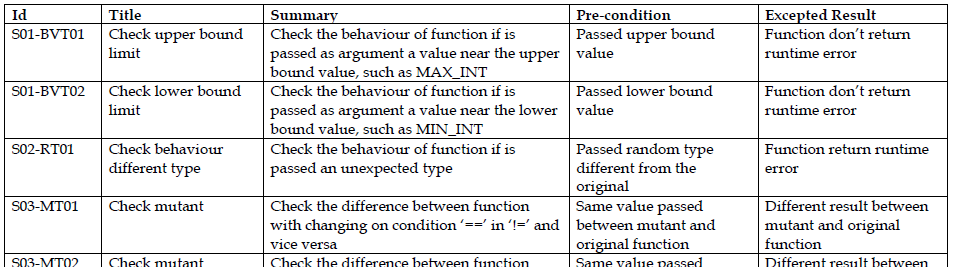
\includegraphics[scale=0.7]{TC.PNG}
  \caption{Esempio di Test Case}
\end{figure}


\item[•] \textit{\textbf{Test Suite}}: sono una raccolta di \textit{Test Case} raggruppati per obiettivi comuni. Una \textit{Test Suite} spesso contiene istruzioni o obiettivi dettagliati per cui sono stati progettati. Contengono anche informazioni sulla configurazione del sistema da utilizzare durante i test.

\begin{figure}[H]
  \centering
  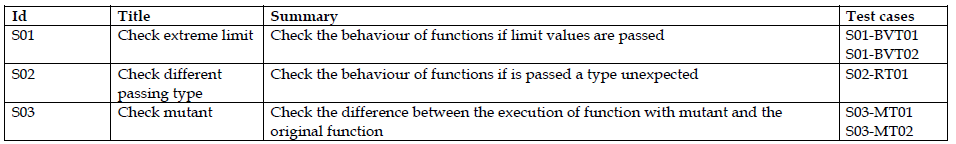
\includegraphics[scale=0.7]{TS.PNG}
  \caption{Esempio di Test Suite}
\end{figure}
\end{itemize}


\subsection{Strumenti utilizzati}
%\textcolor{OliveGreen}{\textbf{Descrivo quali sono gli strumenti e come sono stati implementati}}
I principali strumenti che ho utilizzato e integrato per avere un unico sistema per l'esecuzione automatica dei test previsti per l'analisi dinamica sono:

\begin{itemize}
\item[•] \textbf{CMock}: permette di creare \textit{mock e stub} per testare funzioni dipendenti da altre. Impostando un valore e la rispettiva risposta attesa, si verifica che la funzione in esame svolga correttamente il proprio compito.

\item[•] \textbf{CUnit}: permette di svolgere test di unità, attraverso una serie di asserzioni predefinite fornite da questo strumento. Le asserzioni sono una parte funzionante di codice, da inserire durante la stesura dei test, e si occupano di stabilire se la parte di programma testata funziona correttamente, confrontando il risultato prodotto con un valore imposto dal verificatore.

\item[•] \textbf{Vagrant}: è uno strumento che permette di creare ambienti virtuali temporanei. Questo strumento è necessario in quanto garantisce la ripetibilità dei test. Generando per ogni test un nuovo ambiente, abbiamo infatti la certezza che tutti i test siano svolti nello stesso contesto e nelle medesime condizioni, escludendo quindi eventuali interferenze esterne al programma che possono causare ulteriori errori.
\end{itemize}

\section{Metriche di qualità}
%\textcolor{OliveGreen}{\textbf{Scelte e motivazioni per l'utilizzo di tools di calcolo delle metriche di qualità, associate ad alcune best-practice esistenti.}}

L'ultima fase prevista da questo stage richiedeva la ricerca e la valutazione delle metriche di qualità del software.
Attraverso l'attuazione delle metriche di qualità è possibile definire se il prodotto realizzato è conforme alle aspettative aziendali.

Per garantire un alto livello qualitativo dei processi e per specificare in dettaglio le scelte di progettazione effettuate, ho prodotto un documento denominato \textit{Software quality metrics}.
Lo scopo di questo documento è fornire un valore numerico per alcuni degli attributi di qualità richiesti definiti nel documento \textit{Software quality plan}. La misurazione della qualità del software è utile infatti per identificare eventuali anomalie delle varie componenti software. Mi sono occupato dell'intera stesura del documento, fornendo i dettagli implementativi e, con l'approvazione del responsabile del Reparto di Ricerca e Sviluppo, ho definito i valori di accettazione delle varie metriche.

\subsection{Principi base}
Il principio fondamentale sul quale mi sono basato per trovare delle metriche di qualità è lo standard ISO/IEC 9126.
Questo standard esplora il concetto di qualità del prodotto software dividendo la qualità in interna, esterna e d'uso. Questi tre aspetti di qualità sono fortemente collegati tra loro e alla qualità dei processi.

\begin{figure}[H]
  \centering
  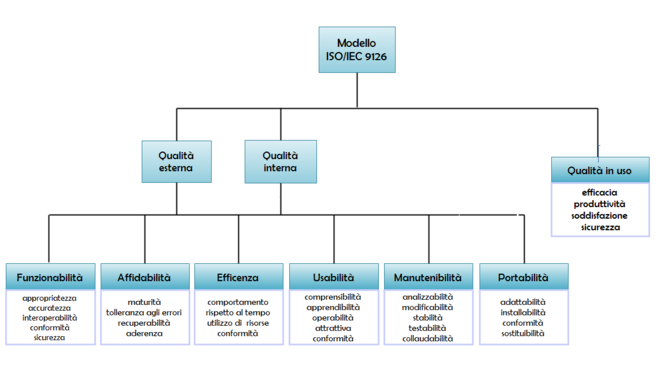
\includegraphics[scale=0.7]{9126.PNG}
  \caption{ISO/IEC 9126 - Divisione della qualità}
\end{figure}

La qualità interna è misurata sui requisiti interni, e considera le componenti interne del prodotto software.

La qualità esterna, invece, si occupa delle caratteristiche esterne, ovvero delle caratteristiche \textit{software} quando questo è eseguito.

La qualità in uso, infine, si occupa di misurare la qualità percepita dall'utente che si trova di fronte al prodotto finito.

Per la qualità interna ed esterna esistono sei caratteristiche principali che devono essere garantite dal prodotto software per aderire a questo standard: funzionalità, affidabilità, efficienza, usabilità, manutenibilità e portabilità.

\subsection{Metriche implementate}
Riporto di seguito alcune delle possibili misurazioni che possono essere effettuate per garantire un prodotto di qualità. Essendo la prima volta che il Reparto di Ricerca e Sviluppo applicava queste metriche, ho deciso di selezionarne solamente alcune. Ho ritenuto opportuno concentrarmi più sui risultati raggiunti che sulla quantità.

\begin{itemize}
\item[•] \textit{Densità di difetti}: è il numero di difetti trovati nel software in un certo periodo di esecuzione. Questa metrica permette di definire se il software può essere rilasciato o meno. La densità di difetti viene conteggiata in rapporto alle linee di codice prodotte. 

\item[•] \textit{Copertura del codice}: questa metrica viene utilizzata per descrivere il grado di copertura dei test rispetto al codice eseguito. Un programma con un alto grado di copertura, misurato in percentuale, garantisce una certa sicurezza, in quanto è stato testato quasi tutto il codice scritto. 

\item[•] \textit{Rapporto difetti trovati e corretti}: questa metrica misura qual è lo stato corrente dell'esecuzione dei test. Tramite questo rapporto si rappresenta la percentuale di miglioramento delle attività di test.

\item[•] \textit{Complessità ciclomatica}: questa metrica misura la complessità con la quale è stato sviluppato il programma. Maggiore è il valore di questa metrica maggiore è la complessità del programma. La complessità ciclomatica indica anche il numero di test che devono essere effettuati per coprire al 100\% il codice sviluppato.

\item[•] \textit{Rapporto linee di codice - linee di commento}: questa metrica indica se il codice è correttamente documentato. Un alto valore di questo rapporto garantisce una buona manutenibilità.
\end{itemize}


Una volta identificate le metriche da calcolare, è necessario definire anche dei valori obiettivo di qualità che si desidera raggiungere. In accordo con il responsabile del Reparto Ricerca e Sviluppo abbiamo definito due range: uno di accettazione, che contiene i valori minimi da raggiungere per considerare il prodotto di qualità, e uno ottimale che contiene i valori richiesti dall'azienda. Di seguito una tabella riassuntiva delle metriche calcolate.
\bigskip

\begin{tabular}{|l l l|}
\hline
Metrica	& Range Accettazione	& Range Ottimale \\
\hline
Densità di difetti & <15\% & <5\% \\
Copertura del codice & <50\% & <90\% \\
Rapporto difetti & <70\% & <90\% \\
Complessità ciclomatica & 0-15 & 0-10 \\
Rapporto linee di codice, commento  & >15\% & >20\% \\
\hline
\end{tabular}

\section{Integrazione delle automazioni}
%\textcolor{OliveGreen}{\textbf{Descrivo come ho fatto per integrare i risultati ottenuti con i sistemi di organizzazione esistenti}}
Dopo aver analizzato e progettato gli strumenti per l'analisi del codice, ho dovuto pianificare attentamente quando e in che modalità eseguire ciò che ho realizzato. 

\begin{figure}[H]
  \centering
  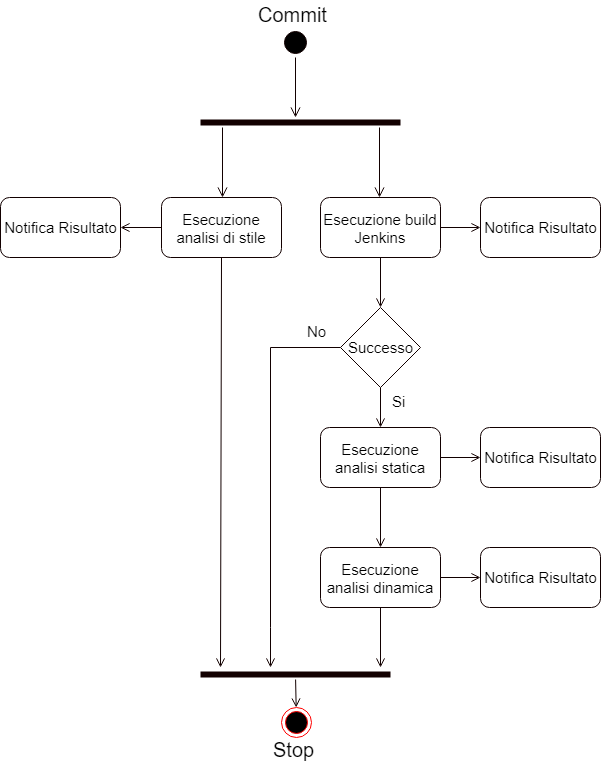
\includegraphics[scale=0.6]{flusso.PNG}
  \caption{Flusso di esecuzione delle automazioni a seguito di un commit}
\end{figure}

L'applicazione degli strumenti di analisi dello stile di codifica viene effettuata tramite gli \textit{hooks} di SVN. 
Con il termine tecnico \textit{hooks}, si intende una serie di script che vengono eseguiti in maniera automatizzata dallo strumento di versionamento utilizzato. Si dividono in due categorie:
\begin{itemize}
\item[•] \textit{pre-commit}: lo \textit{script} viene eseguito prima del salvataggio delle modifiche sulla \textit{repository}. Il salvataggio viene effettuato solamente se il risultato dello script ha prodotto un esito positivo, altrimenti viene notificato allo sviluppatore un report con le motivazioni del fallimento.

\item[•] \textit{post-commit}: lo \textit{script} viene eseguito a seguito del salvataggio sulla \textit{repository} delle modifiche effettuate. Questa tipologia di \textit{script} non vincola il caricamento dei file, ma notifica soltanto l'esito dell'esecuzione.
\end{itemize}

Le regole sullo stile di codifica sono state definite ed implementate in un secondo momento rispetto alla prima e principale stesura del codice. Per non scoraggiare gli sviluppatori, rifiutando la maggior parte dei \textit{commit} contenenti molti errori pregressi ho deciso, in accordo con il responsabile e in linea con quanto pianificato lo scorso anno, di mantenere la tecnica di esecuzione degli strumenti tramite l'utilizzo dei \textit{post-commit hooks}. In questo modo gli sviluppatori possono lavorare senza grossi vincoli, ma con la consapevolezza di dover migliorare lo stile di scrittura. 

Sul \textit{client} SVN utilizzato, a termine del caricamento delle modifiche effettuate, viene visualizzato un report con tutte le tipologie di errori riscontrate durante l'analisi dei file modificati o creati.

\begin{figure}[H]
  \centering
  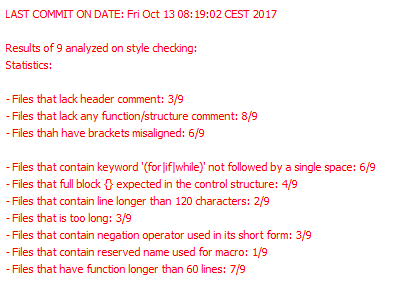
\includegraphics[scale=0.8]{style.PNG}
  \caption{Esempio report post-commit}
\end{figure}

In coda a questo messaggio di riepilogo degli errori riscontrati viene visualizzato un \textit{link} che rimanda ad un report più dettagliato. In questo report vengono visualizzati tutti i file analizzati con i riferimenti al numero della riga in cui è stato trovato l'errore, in questo modo è possibile, in modo facilitato, trovare e correggere manualmente la non conformità segnalata.

\bigskip

Parallelamente a questa analisi, vengono eseguiti dal server anche gli strumenti realizzati per l'analisi statica e dinamica.

L'applicazione degli strumenti di analisi statica viene dunque effettuata automaticamente, a seguito di ogni \textit{commit}, tramite il sistema di integrazione continua \textit{Jenkins}, solamente se la compilazione di tutto il \textit{software} è stata portata a termine senza alcun errore.

L'esecuzione delle regole di conformità di MISRA C è stata eseguita in un ambiente diverso rispetto a quello dell'esecuzione degli altri strumenti. Questo strumento, fornito internamente all'IDE IAR System, ne richiedeva l'esecuzione su un sistema operativo \textit{Windows}, e non \textit{Linux}, come tutti gli altri strumenti utilizzati. È stato necessario dunque utilizzare due server distinti per garantire l'esecuzione completa di quanto pianificato per l'analisi statica, e uno strumento che permettesse la comunicazione diretta e immediata tra i due sistemi operativi. Ho quindi utilizzato la tecnologia SSH per lo scambio dei report di analisi dei file analizzati.

\begin{figure}[H]
  \centering
  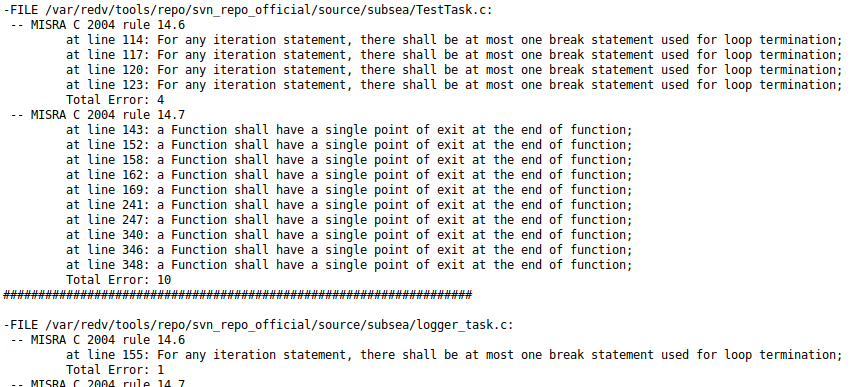
\includegraphics[scale=0.6]{static1.PNG}
  \caption{Esempio report analisi statica}
\end{figure}

L'esecuzione degli strumenti di analisi dinamica viene effettuata come ultima operazione automatizzata di \textit{Jenkins}.

Diversamente da quanto è stato pianificato, l'utilizzo dello strumento \textit{Vagrant} non è andato a buon fine in quanto ho avuto delle difficoltà inattese con la virtualizzazione annidata richiesta dallo strumento, ma non disponibile sul server utilizzato.

Si sono verificati numerosi problemi durante l'esecuzione dei test sull'intero prodotto software realizzato, in quanto il progetto \textit{Subsea} utilizza compilatore IAR, mentre gli strumenti CMock e CUnit utilizzano il compilatore gcc. Ho preferito dunque effettuare un'analisi approfondita e teorica delle varie tecniche di analisi, applicando quanto studiato su una piccola porzione di progetto modificata e resa compatibile con gcc, per far vedere che comunque la realizzazione dei test è fattibile.

\bigskip
Il calcolo delle metriche, viene invece eseguito quotidianamente ed in modo automatico da \textit{Jenkins}.

La misurazione delle metriche di qualità attraverso gli strumenti di analisi è divisa in due fasi. 

Nella prima fase gli strumenti analizzano i report generati durante l'attività di analisi dinamica, in modo tale da garantire un valore numerico sui risultati dell'esecuzione dei test. In questa fase vengono generati i risultati delle metriche associate ai test, come la densità di difetti o la copertura del codice.

Nella seconda fase poi, vengono calcolate le metriche che non richiedono l'esecuzione del software. Alcuni esempi di metriche calcolate in questa fase sono la complessità ciclomatica, e il rapporto tra linee di codice e linee di commento.

Queste metriche vengono calcolate dopo la terminazione delle procedure di analisi dinamica in modo automatizzato dal sistema di integrazione continua \textit{Jenkins.}

Il report che viene visualizzato contiene  sia dei dei valori medi complessivi che indicano lo stato qualitativo dell'intero prodotto, sia dei valori specifici per i singoli file analizzati.

\begin{figure}[H]
  \centering
  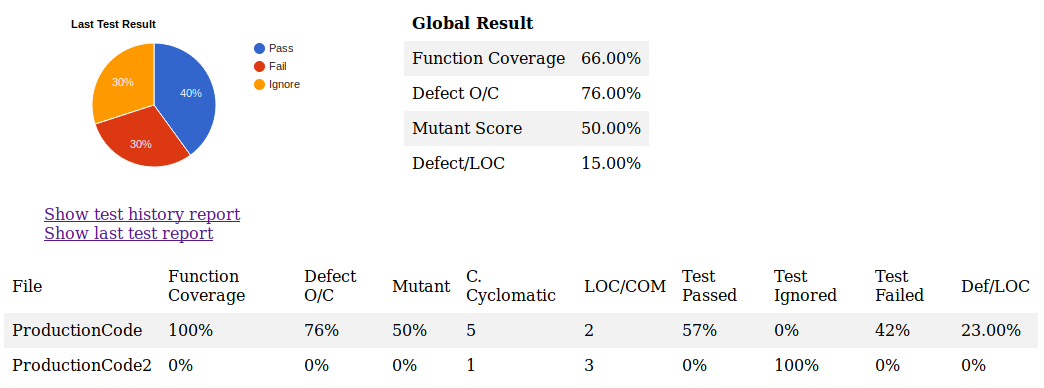
\includegraphics[scale=0.5]{metricReport.PNG}
  \caption{Report calcolo metriche}
\end{figure}
%############################################################################################
\bigskip

Una volta creati tutti gli strumenti per coprire le richieste del progetto riguardanti analisi dello stile, analisi statica, analisi dinamica e calcolo delle metriche di qualità, mi sono reso conto che i report generati contenenti i risultati di queste attività erano sparsi, difficili da raggiungere ed eccessivamente verbosi.

Dalla figura 3.9 si può vedere che il report che visualizza i risultati di analisi statica è contenuto in un unico file di testo, e vengono visualizzati tutti gli errori segnalati. In questo caso è veramente difficile e costoso in termini di tempo trovare un particolare tipo di errore segnalato. Ho così deciso, in accordo con il \textit{tutor} aziendale, di creare un nuovo componente aggiuntivo sul sistema di gestione di processo Redmine, fornendo un unico punto di accesso per tutti i report prodotti.

In questo modo, sfruttando le potenzialità di Redmine, ho potuto gestire gli errori segnalati all'interno di una base di dati, nella quale è possibile ricercare e filtrare i risultati a proprio piacimento.

\begin{figure}[H]
  \centering
  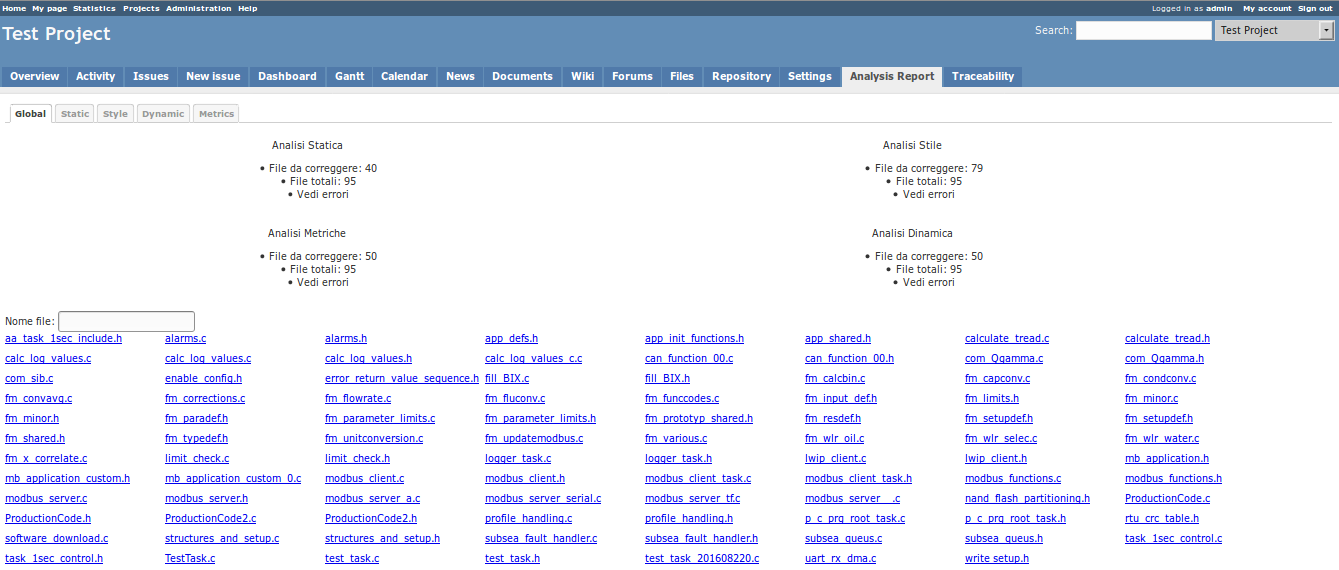
\includegraphics[width=420px]{image009.png}
  \caption{Componente integrato con Redmine - Ricerca per file}
\end{figure}

\begin{figure}[H]
  \centering
  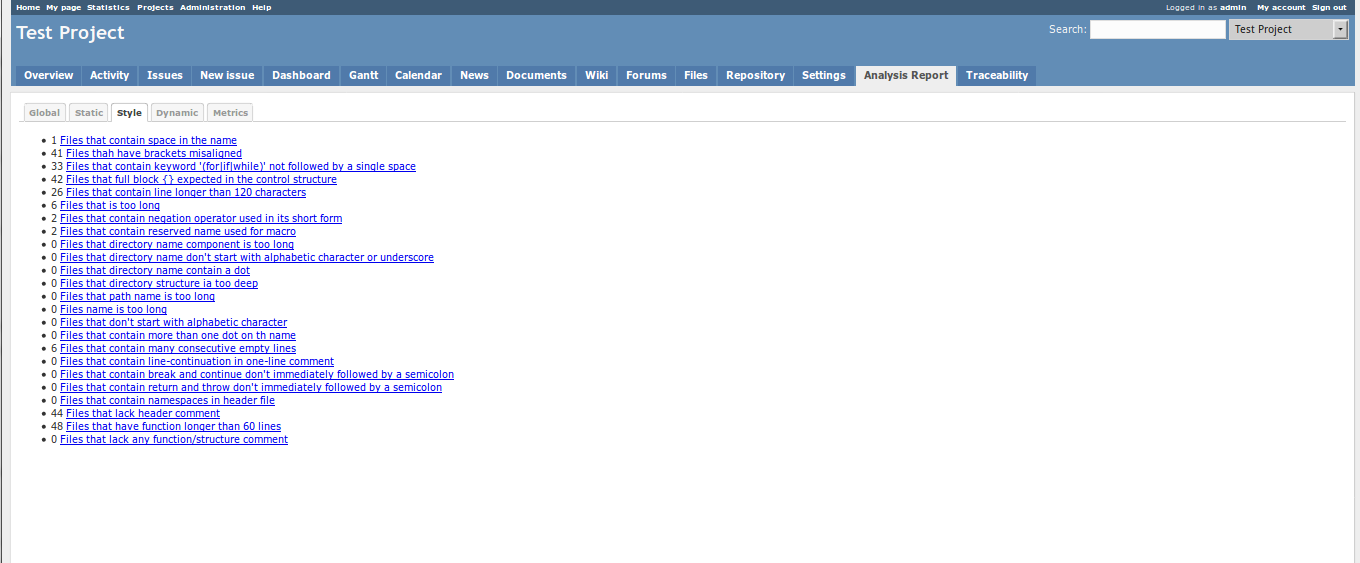
\includegraphics[width=420px]{image012.png}
  \caption{Componente integrato con Redmine - Ricerca per segnalazioni stile di codifica}
\end{figure}

\section{Conclusioni}
Le attività descritte fino a qui sono state portate tutte a termine nei tempi previsti.

Sono stati soddisfatti tutti gli obiettivi minimi previsti e quasi tutti gli obiettivi massimi.

Sono riuscito ad applicare alla totalità dei file prodotti dagli sviluppatori, le tecniche di analisi dello stile di codifica e di analisi statica. In particolare, ho integrato i risultati forniti dagli strumenti realizzati sia con i sistemi di versionamento, sia con i sistemi di gestione di processi. L'integrazione con i sistemi di versionamento serviva a dare la possibilità
al programmatore di visionare immediatamente le eventuali non conformità derivati dall'analisi dello stile di codifica, invece l'integrazione con i sistemi di gestione dei processi, attraverso la realizzazione del componente aggiuntivo per Redmine, dava una rapida visione degli esiti delle analisi effettuate.

Per quanto riguarda gli obiettivi massimi, associati all'analisi dinamica, invece, non sono riuscito a soddisfarli tutti pienamente. Questo perché, alla luce dei problemi sopra descritti (Vedi 3.6), derivanti dall'incompatibilità tra gli strumenti di analisi trovati e il compilatore IAR utilizzato dall'azienda, non è stato possibile definire una \textit{Test Suite} con copertura almeno del 50\%. Ho comunque realizzato alcuni test su frammenti di programma, potendo così dimostrare l'efficacia e la potenza di questo tipo di analisi.


%\section{Documenti prodotti}
%Per garantire un alto livello qualitativo di tutti i processi implementati, ho prodotto una serie di documenti che specificano in dettaglio le scelte effettuate durante la realizzazione degli strumenti, e forniscono tutti i dettagli implementativi necessari per una futura manutenzione del codice che ho scritto.
%Tutta la documentazione è stata scritta in lingua inglese.
%
%\paragraph*{Software quality plan}
%Questo documento è il documento principale che racchiude tutte le tecniche e procedure per garantire un alto livello di qualità del software. Ha come scopo la definizione di procedure, tecniche e strumenti coinvolti nel garantire la qualità del software prodotto.
%
%Questo documento era già stato redatto nel precedente stage, mi sono occupato di revisionarlo, aggiungendo una specifica più dettagliata sulla gestione delle misure, e mi sono occupato dell'indicizzazione degli altri documenti ad esso associati.
%
%\paragraph*{Code style guide}
%
%
%\paragraph*{Code static analysis}
%.
%
%\paragraph*{Code dynamic analysis}
%
%
%\paragraph*{Software quality metrics}
